\documentclass[openany, 11pt]{book}

% ============== PACKAGES ==============
\usepackage{graphicx}       % For including images
\usepackage{fancyhdr}       % For customizing headers and footers
\usepackage{titlesec}       % For formatting section and chapter titles
\usepackage{textcase}       % For text case transformations
\usepackage{ulem}           % For underlining and strikeout text
\usepackage{tcolorbox}      % For creating colored/text-boxes
\usepackage{courier}        % For using Courier as a font
\usepackage[margin=2.5cm, top=2cm]{geometry} % Set general page margins
\usepackage{background}     % For adding a background box on each page
\usepackage{etoolbox}       % For resetting counters
\usepackage[ngerman, english, dutch]{babel}
\usepackage{iflang}
\usepackage{enumitem}
\usepackage{subcaption}
\usepackage{makecell}
\usepackage{mdframed}
\usepackage{amsmath}
\usepackage{csquotes}

% ============ GENERAL SETTINGS ============
\renewcommand{\rmdefault}{pcr} % Set Courier as the default font family
\graphicspath{{./}{./images/}} % Define paths for images

% ============ PAGE NUMBERING ============
\makeatletter
\renewcommand{\thepage}{%
  \thechapter.%                % Include the chapter number
  \ifnum\c@section<10 0\fi%    % Add leading zero to single-digit section numbers
  \@arabic\c@section-%         % Render section number
  \arabic{page}%               % Render the page number
}
\makeatother

% Reset section page numbers per chapter
\newcounter{sectioninchapter}
\pretocmd{\chapter}{\setcounter{sectioninchapter}{0}}{}{}
\pretocmd{\section}{%
  \ifnum\value{sectioninchapter}=0
    \setcounter{page}{1}
  \else
    \clearpage\setcounter{page}{1}
  \fi
  \stepcounter{sectioninchapter}
}{}{}

% ============= HEADER CONFIG =============
\setlength{\topmargin}{-2cm}      % Move content block closer to the top
\setlength{\headheight}{33pt}     % Increase header height to fit the logo
\setlength{\headsep}{10pt}        % Space between the header and content

\pagestyle{fancy}
\fancyhf{} % Clear default header/footer content
\fancyhead[L]{
\includegraphics[height=1cm]{maho-logo.png}} % Add logo on the left
\fancyhead[C]{\raisebox{1.2\height}{\textbf{MH 400 E}}}    % Add centered header text
\fancyhead[R]{\raisebox{1.2\height}{\textbf{\thepage}}}    % Add page number on the right
\renewcommand{\headrulewidth}{0pt} % Remove header rule line

% Header for chapter title pages
\fancypagestyle{plain}{%
  \fancyhf{}
  \fancyhead[L]{
\includegraphics[height=1cm]{maho-logo.png}}
  \fancyhead[C]{\raisebox{1.2\height}{\textbf{MH 400 E}}}
  \fancyhead[R]{\raisebox{1.2\height}{\textbf{\thepage}}}
}

% ========== BACKGROUND CONFIG ==========
\backgroundsetup{%
  scale=1,
  color=black,
  opacity=1,
  angle=0,
  position=current page.south west,
  vshift=1cm,
  hshift=2cm,
  nodeanchor=south west,
  contents={%
    \begin{tikzpicture}[remember picture, overlay]
      \node[anchor=south west, inner sep=0] (box) at (0, 0) {
        \begin{tcolorbox}[
          colframe=black, 
          colback=white, 
          boxrule=0.5mm,
          sharp corners, 
          width=\dimexpr\paperwidth-3cm\relax,
          height=\dimexpr\paperheight-3cm\relax
        ]
        \end{tcolorbox}
      };
      \draw[black, thick] ([yshift=1cm]box.south west) -- ([yshift=1cm]box.south east);
      \node[anchor=south, yshift=-.6cm] at ([yshift=1cm]box.south) {
        \footnotesize \textit{MAHO WERKZEUGMACHINENBAU BABEL \& CO. D-8962 FRONTEN}
      };
    \end{tikzpicture}
  }
}

% ========== CHAPTER FORMATTING ==========
\titleformat{\chapter}[block]{\normalfont\Large\bfseries}{}{0pt}{\chapterTitleStyle}
\titlespacing*{\chapter}{0pt}{0pt}{20pt}
\newcommand{\chapterTitleStyle}[1]{%
  \vspace{-1em}
  \underline{\MakeUppercase{#1}}
  \vspace{1em}
}
\setcounter{chapter}{-1} % Start chapter numbering at 0

% ========== SECTION FORMATTING ==========
\titleformat{\section}[block]{\normalfont\large\bfseries}{}{0pt}{\sectionTitleStyle}
\titlespacing*{\section}{0pt}{10pt}{10pt}
\newcommand{\sectionTitleStyle}[1]{%
  \underline{\MakeUppercase{#1}}
}

% ======== SUBSECTION FORMATTING =========
\titleformat{\subsection}[block]{\normalfont\normalsize\bfseries}{}{0pt}{}
\titlespacing*{\subsection}{0pt}{10pt}{10pt}

% Define commands for easier switching
\newcommand{\DE}[1]{\foreignlanguage{ngerman}{#1}} % Short for German
\newcommand{\EN}[1]{\foreignlanguage{english}{#1}} % Short for English
\newcommand{\NL}[1]{\foreignlanguage{dutch}{#1}}   % Short for Dutch

% =========== LIST FORMATTING =============
\renewcommand{\labelitemi}{-}
\setlist[itemize,1]{left=0pt}

% =========== CUSTOM COMMANDS =============
\newcommand{\notebox}[2]{%
    \noindent
    \begin{minipage}[t]{2cm} % Label in a 2cm-wide top-aligned box
        \textbf{#1:}
    \end{minipage}%
    \hspace{0.5em}% Small horizontal space between label and text
    \begin{minipage}[t]{\dimexpr\textwidth-2.5cm\relax} % Remaining width for the body
        #2
    \end{minipage}%
    \vspace{1em} % Adjust the spacing as needed
}

\newcommand{\infoBullet}[2]{\noindent $\bullet$ #1, see Page #2.}

\newcommand{\sectionLikeSubsection}[1]{%
    \newpage
    \subsection{\MakeUppercase{\textbf{\uline{#1}}}}
}

% =========== DOCUMENT CONTENT ===========
\begin{document}

\refstepcounter{chapter}
\addcontentsline{toc}{chapter}{INHALTSVERZEIGNIS}

\thispagestyle{coverpage}

\begin{titlepage}
    \thispagestyle{coverpage}

    \vspace*{0cm}

    {\sffamily

        \noindent
        \begin{tabularx}{\textwidth}{X r}
            
\includegraphics[height=1.5cm]{maho-logo.png} &
            {\Huge \textbf{Operator's Manual}} \\
            \multicolumn{2}{l}{\rule{\textwidth}{0.4mm}} \\
            & {\normalsize Nr. 76.34521}
        \end{tabularx}

        \centering
        \vspace{2cm}

        {\fontsize{60pt}{62pt} \bfseries MH400E}\\[1cm]

        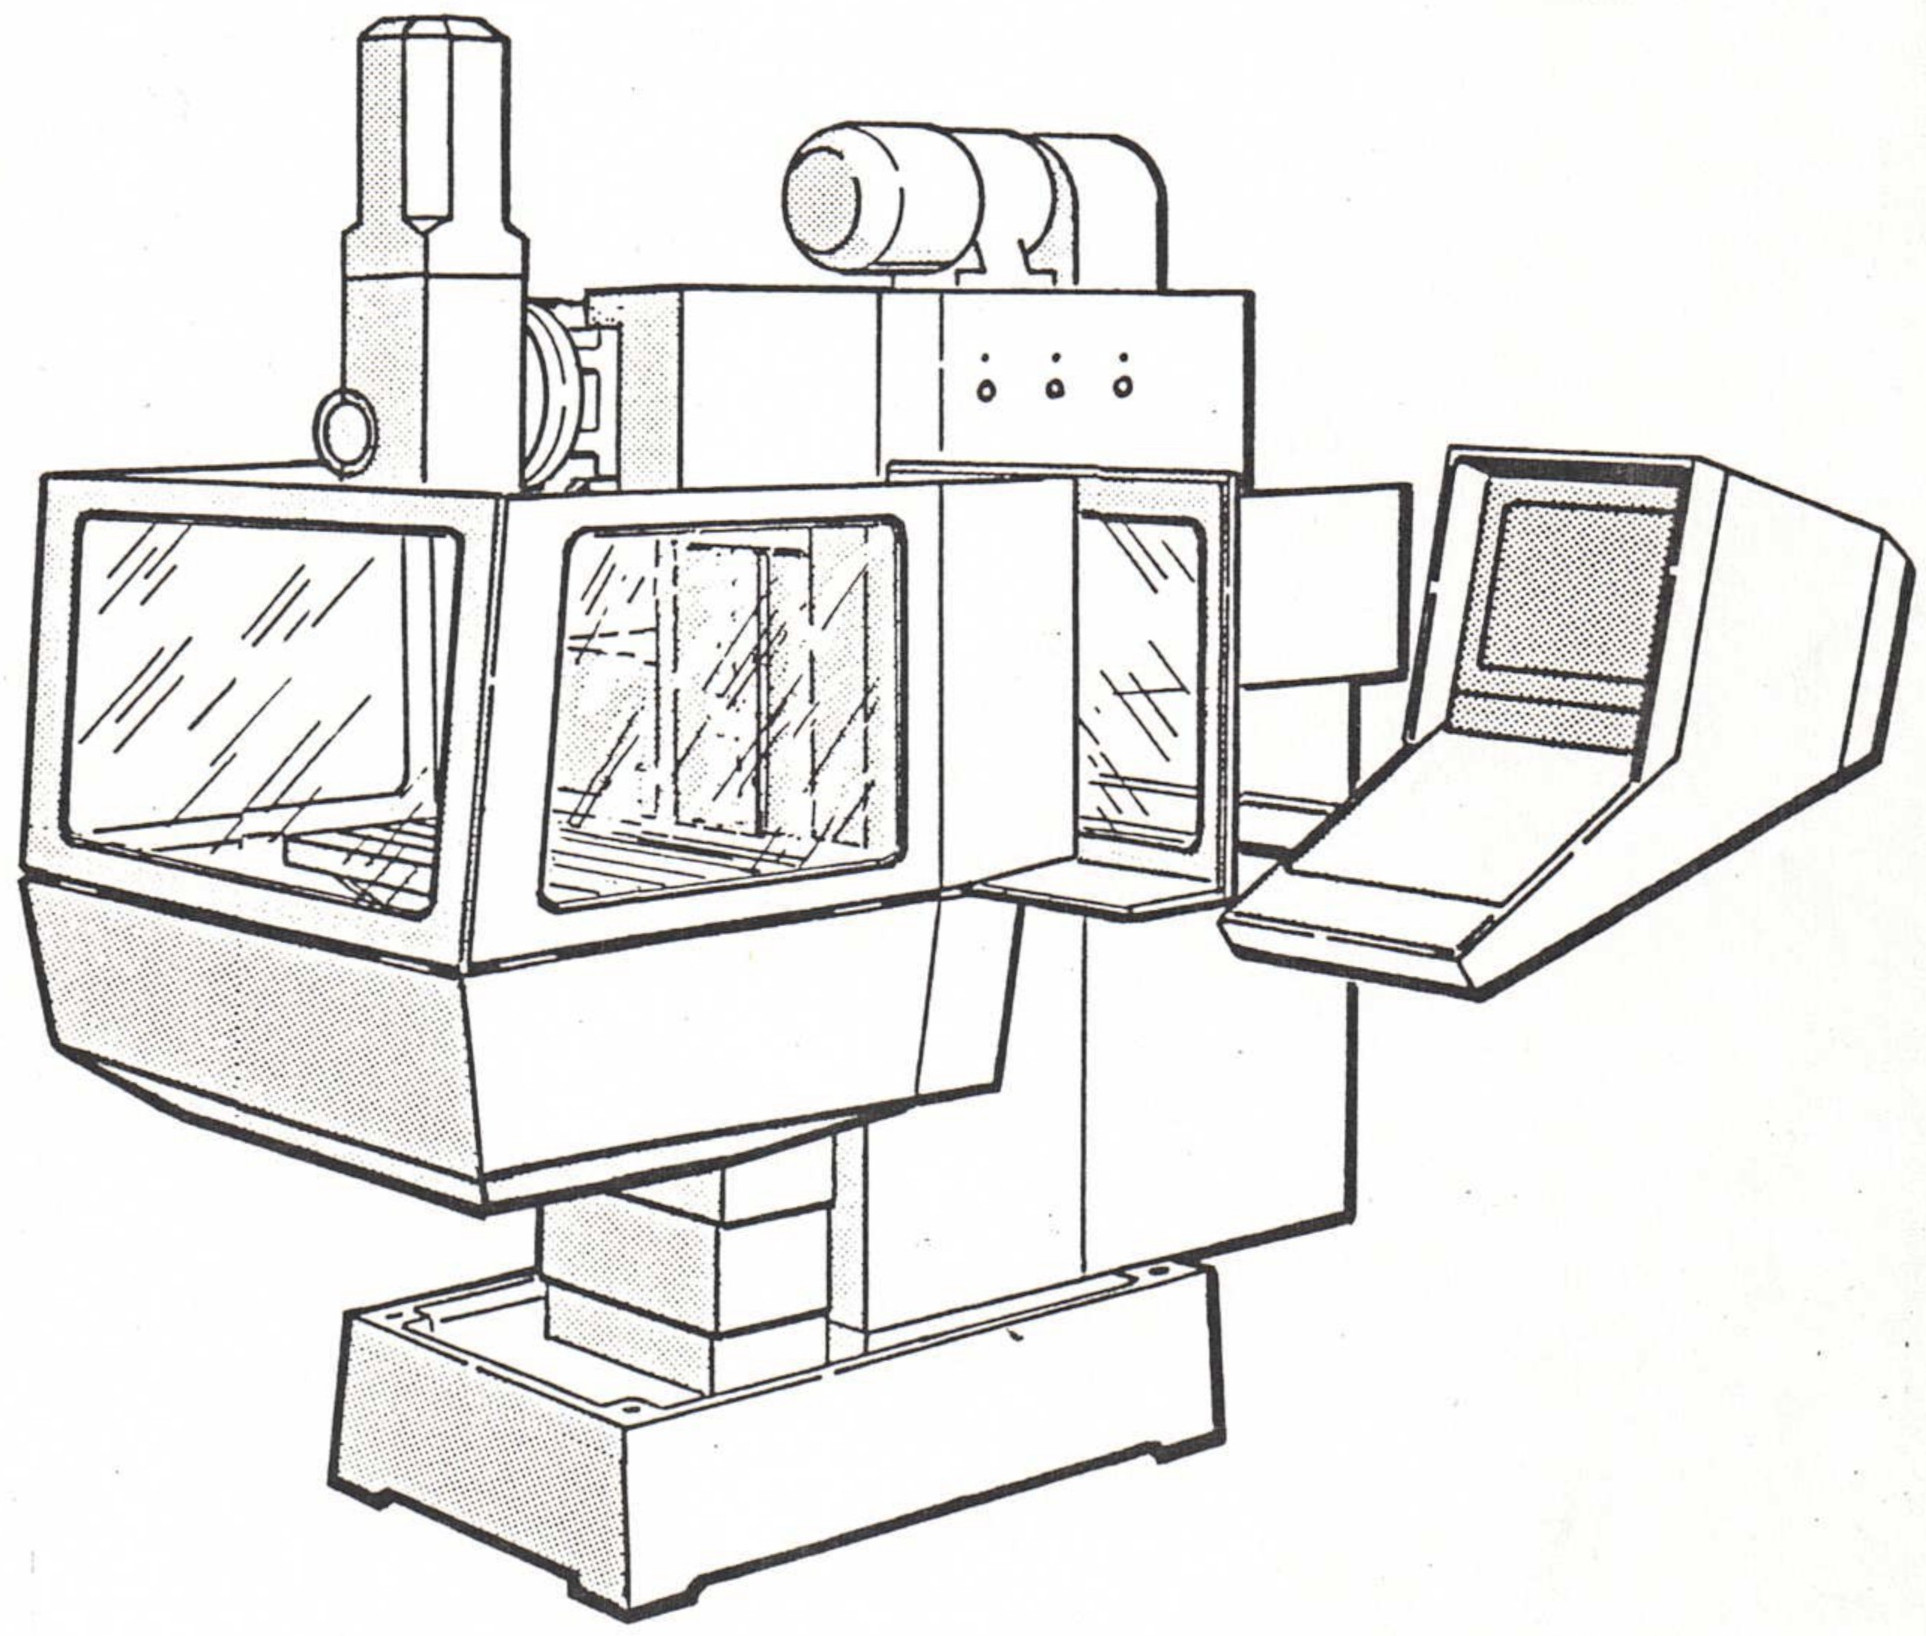
\includegraphics[width=0.9\textwidth]{chapter0/cover-image.jpg} 

        \vfill

         \noindent
         \begin{center}
             \parbox{\textwidth}{\centering {\Huge \textbf{Operation - Maintenance - Repair}}}
         \end{center}
    }
\end{titlepage}

\clearpage % Move to the next page and resume normal styling
\pagestyle{fancy} % Re-enable the default layout

\setsectiontitle{To our customers}
\setcounter{chapter}{0}
\setcounter{section}{0}

This operator's manual contains the essential information required for the proper operation and maintenance of your MAHO machine tool. It belongs in the hands of the operating and maintenance personnel.

The present operator's manual includes the separate operating instructions for CNC 432/10 graphics, the programming instructions for CNC 432 of the control unit, the programming manual for the \enquote{Geometry Package}, and the folder \enquote{Assembly Drawings and Parts Lists}.

Tax-specific details are listed \textbf{only} in the operating manual for CNC 432/10 graphics and should be referenced there.

The machine may only be put into operation after the operating and maintenance personnel have carefully read the operator's manual and have thoroughly\\ familiarized themselves with all details.

Operation and maintenance of the machine must be carried out in accordance with the instructions provided in this operator's manual.

\notebox{NOTE}{\textbf{We assume no liability for damages resulting from failure to follow these instructions or from improper handling.}}

If malfunctions occur that cannot be resolved independently, the cause of the malfunction should be determined using the operator's manual before \\contacting the appropriate MAHO representative or the MAHO company.

This operator's manual is designed to help you complete your machining tasks efficiently. We are confident that the delivered MAHO machine tool will fully meet your expectations. \\[1cm]

\noindent
\textbf{\textcopyright\ Copyright} \\[0.2cm]

This technical manual may \textbf{not}, even in part, be reproduced or made accessible to third parties without the express permission of the publisher.

\newpage

\subsection{Page Numbering}

The pages of this manual are numbered sequentially within each chapter \\according to sections. The page numbers are displayed in the upper right corner and are structured so that the page number follows the section number.

\textbf{EXAMPLE}: \texttt{3.20-3}, means Chapter 3, Section 20, Page 3.

If expansions occur within a section, these are numbered using the page number of the previous page followed by the numbers 1, 2, 3, etc., separated by a period.

\textbf{EXAMPLE}: \texttt{3.20-3.1}, means Chapter 3, Section 20, Page 3, Supplementary Page 1.

Figures and tables are not separately numbered.

The position numbers in the figures refer to the content of the section and can span 2-3 figures.

If positions of a figure are referenced in the text, they are placed within parentheses \texttt{()}.

\subsection{Notices in this Manual}

The following notices are used in this manual:

\notebox{NOTICE}{Applies to technical details that the user must observe.}

\notebox{CAUTION}{Applies to work or operational procedures that must be followed precisely to prevent damage or destruction of the system.}

\notebox{WARNING}{Applies to work or operational procedures that must be followed precisely to prevent hazards to personnel. This also includes \textbf{CAUTION}.}

\subsection{Cross-References}

To avoid redundant descriptions, content-related connections are established in this manual using cross-references.

\textbf{EXAMPLE}:
\begin{quote}
\noindent \hspace{-0.25cm} .... according to instructions .... \\
\hspace{1.3cm} .... see Sheet/Page ....
\end{quote}

\subsection{Location Definition}

The designations front, back, left, right, top, and bottom are based on the perspective from the spindle head looking toward the workpiece.

\setsectiontitle{Table of Contents}
\renewcommand{\arraystretch}{1.3} % Adjust row spacing for readability

\begin{tabularx}{\textwidth}{X r}
    \textbf{\underline{Commissioning the Machine}} & \\ % Main Section (No page number)
    Important Notes \dotfill & 1.01-1 \\
    Transport of the Machine \dotfill & 1.02-1 \\
     & 1.02-2 \\ % No extra &
    Setting Up the Machine \dotfill & 1.03-1 \\
     & 1.03-2 \\
     & 1.03-3 \\
    Setup Plan and Workspace Layout \dotfill & 1.04-1 \\
    Dimensional Drawing of the Machine \dotfill & 1.05-1 \\
    Removal of Rust Protection Agent \dotfill & 1.08-1 \\
    Spindle head oil fill \dotfill & 1.09-1 \\
    Connecting to the Electrical Network \dotfill & 1.10-1 \\
    Commissioning Checklist \dotfill & 1.11-1 \\[0.5cm]

    \textbf{\underline{General Description of the Machine}} & \\ % Main Section
    Technical Data \dotfill & 2.01-1 \\
     & 2.01-2 \\
    Machine Overview \dotfill & 2.02-1 \\
    Component Identification \dotfill & 2.02-2 \\
     & 2.02-3 \\
     & 2.02-4 \\
     & 2.02-5 \\
     & 2.02-6 \\
     & 2.02-7 \\
     & 2.02-8 \\
    Motion Directions \dotfill & 2.03-1 \\
    Control Station \dotfill & 2.04-1 \\
     & 2.04-2 \\
    Hand Control Panel \dotfill & 2.04-5 \\
    Gear Train Schematic \dotfill & 2.10-1 \\
    Main Gearbox \dotfill & 2.10-2 \\[0.5cm]

    \textbf{\underline{Machine Operation}} & \\
    Functional Testing - Trial Run \dotfill & 3.01-1 \\
     & 3.01-2 \\[0.5cm]
\end{tabularx}

\newpage

\begin{tabularx}{\textwidth}{X r}
    Manual Spindle Speed Selection \dotfill & 3.03-2 \\
    Horizontal Working Spindle \dotfill & 3.04-1 \\
    Horizontal Milling with Counter Holder \dotfill & 3.05-1 \\
    Horizontal to Vertical Conversion \dotfill & 3.07-1 \\
    Vertical to Horizontal Conversion \dotfill & 3.08-1 \\
    Vertical Milling Head without Quill Feed \dotfill & 3.09-1 \\
    Automatic Tool Clamping \dotfill & 3.12-1 \\
    Reworking of Standard Tool Shafts \dotfill & 3.13-1 \\
    Tool Shaft According to DIN 69871 \dotfill & 3.13-3 \\
    Manual Adjustment of the Machine Slide \dotfill & 3.15-2 \\
    Hydraulic Plan and Equipment List \dotfill & 3.18-1 \\
    Hydraulic System \dotfill & 3.18-3 \\
    Automatic Central Lubrication System \dotfill & 3.20-1 \\
    Equipment List - Automatic Central Lubrication \dotfill & 3.20-2 \\
    Automatic Central Lubrication \dotfill & 3.20-3 \\
     & 3.20-4 \\
     & 3.20-5 \\
    Coolant System \dotfill & 3.22-1 \\
    Splash Protection \dotfill & 3.24-1 \\[0.5cm]

    \textbf{\underline{Worktables}} & \\
    Fixed Angle Table \dotfill & 4.01-1 \\
     & 4.01-2 \\
    Universal Rotary Table \dotfill & 4.03-1 \\
     & 4.03-2 \\
     & 4.03-3 \\
     & 4.03-4 \\
     & 4.03-5 \\
     Angle Adjustment Display for B-Axis \dotfill & 4.04-1 \\[0.5cm]
\end{tabularx}

\newpage

\begin{tabularx}{\textwidth}{X r}
    \textbf{\underline{CNC Control}} & \\ % Main Section (No page number)
    Linear Measurement Systems and Display Units \dotfill & 5.01-1 \\
    Machine Constants CNC 432 \dotfill & E3.21741C \\
     & E3.21742C \\
     & E3.21743C \\
     & E3.21744C \\
     & E3.24628C \\
     & E3.24629C \\
     & E3.24630C \\
    Error List CNC 432 \dotfill & E3.22870C \\
     & E3.22871C \\
     & E3.22872C \\
     & E3.25024C \\
    Operating Manual CNC 432/Graphics \dotfill & 76.00471 \\
    Geometry Package for CNC 432/Graphics \dotfill & 76.00461 \\
    Programming Manual CNC 432 \dotfill & 76.00211 \\[0.5cm]

    \textbf{\underline{Accessories}} & \\ % Main Section
    High-Speed Milling Spindle \dotfill & 6.02-1 \\
    Dot-Matrix Printer ZIP 30 (Separate Manual) \\[0.5cm] % No page number

    \textbf{\underline{Maintenance}} & \\ % Main Section
    Important Notes \dotfill & 7.01-1 \\
    Machine Lubrication Plan \dotfill & 7.02-1 \\
    Lubrication Schedule \dotfill & 7.03-1 \\
    Lubricant Recommendations \dotfill & 7.06-1 \\
     & 7.06-2 \\
    Coolants \dotfill & 7.07-1 \\
     & 7.07-2 \\
     & 7.07-3 \\
     & 7.07-4 \\[0.5cm]
\end{tabularx}

\newpage

\begin{tabularx}{\textwidth}{X r}
    Removing the Machine Covers \dotfill & 7.10-1 \\
    Maintenance Plan \dotfill & 7.20-1 \\
    Overview of Maintenance Tasks for Mechanics and Hydraulics \dotfill & 7.21-1 \\
    Overview of Maintenance Tasks for Electrical and Electronics \dotfill & 7.22-1 \\
    Special Tools for Maintenance and Servicing \dotfill & 7.23-1 \\
    Adjusting the Gibs \dotfill & 7.30-1 \\
    Guideway Wiper Maintenance \dotfill & 7.31-1 \\
    Replacing the Feed Drive Timing Belt \dotfill & 7.33-1 \\
     & 7.33-2 \\
     & 7.33-3 \\
     & 7.33-5 \\
    Installation and Maintenance of the Poly-V Belt \dotfill & 7.34-1 \\
     & 7.34-2 \\
    Adjusting the Collet for Automatic Tool Clamping \dotfill & 7.35-1 \\
     & 7.35-2 \\
    Readjustment Work on the Universal Rotary Table \dotfill & 7.40-1 \\
     & 7.40-2 \\
    Maintenance of DC Motors \dotfill & 7.60-1 \\
     & 7.60-2 \\
     & 7.60-3 \\
    Maintenance of Three-Phase Motors \dotfill & 7.61-1 \\[0.5cm]

    \textbf{\underline{Spare Parts Plans and Lists}} & \\ % Main Section
    Notes on Ordering Spare Parts \dotfill & 8.00-1 \\
    Spare and Wear Parts List \dotfill & 99.34504 \\[0.5cm]

    \textbf{\underline{Disassembly Instructions}} & \\ % Main Section
    Main Motor \dotfill & 9.01-1 \\
    Replacing the Feed Motor \dotfill & 9.08-1 \\
     & 9.08-2 \\
     & 9.08-3 \\
\end{tabularx}

\notebox{NOTE}{The mandatory machine constants for the machine are supplied as punched tape and plaintext. They are located with the electrical circuit diagrams in the control cabinet of the machine.}

\refstepcounter{chapter}
\addcontentsline{toc}{chapter}{Before Starting the Machine}

\section{Important Notes}

\subsection{Factory Number}
\begin{itemize}
    \item The information in this operator's manual applies \uline{\textbf{only}} to the machine whose factory number is stamped on the machine's nameplate.
    \item For all inquiries and spare part orders, the factory number of the machine must be specified.
    \item If inquiries pertain to a specific page of the operator's manual, the page number must also be provided.
\end{itemize}

\subsection{Before Starting the Machine}
\begin{itemize}
    \item Carefully read the operator's manual.
    \item Set up the machine (see Page 1.03-1).
    \item Ensure that the machine has reached room temperature.
    \item Remove rust protection (see Page 1.08-1).
    \item Tighten all terminal screws on the terminal strips, contactors, relays, and fuses in the control cabinet; they may have loosened due to vibrations during transport.
    \item Connect the machine to the electrical network (see Page 1.10-1).
    \item Check oil levels (see Page 7.02-1 and 7.03-1).
    \item Fill the machine with coolant (see Page 3.22-1).
\end{itemize}

\subsection{Interlocks of the Machine}
\begin{itemize}
    \item After switching off the main switch -Q1- in the control cabinet and after every power failure, the machine must be restarted.\footnotemark[1]
    \item The red mushroom button of the EMERGENCY STOP switch must not be pressed during this process.
    \item After each EMERGENCY STOP, the corresponding mushroom button must be \\released by turning it clockwise, and the machine must be restarted.\textsuperscript{\footnotemark[1]}
\end{itemize}

\footnotetext[1]{"Start the machine", see separate CNC 432 operating instructions.}

\section{Transport of the Machine}

The dimensions and weights of the machine with the fixed table and coolant container are as follows:

\begin{table}[h]
\centering
\begin{tabular}{lll}
\textbf{Packaging Type} & \makecell{\textbf{Dimensions}\\\textbf{(L x W x H) [m]}} & \textbf{Weight [kg]} \\ \hline
EURO Packaging (Pallet/Carton) & $1.9 \times 1.8 \times 2$ & 1450 \\
Box (USSR) & $1.9 \times 1.9 \times 2.05$ & 1590 \\
Box (Seaworthy) & $2.35 \times 1.9 \times 2.05$ & 1693 \\
Container Loading (Machine on Pallet) & $1.8 \times 1.8 \times 1.98$ & 1362 \\
\end{tabular}
\end{table}

\begin{figure}[h]
    \centering
    \begin{minipage}[b]{0.35\textwidth} % Align to the bottom with [b]
        \centering
        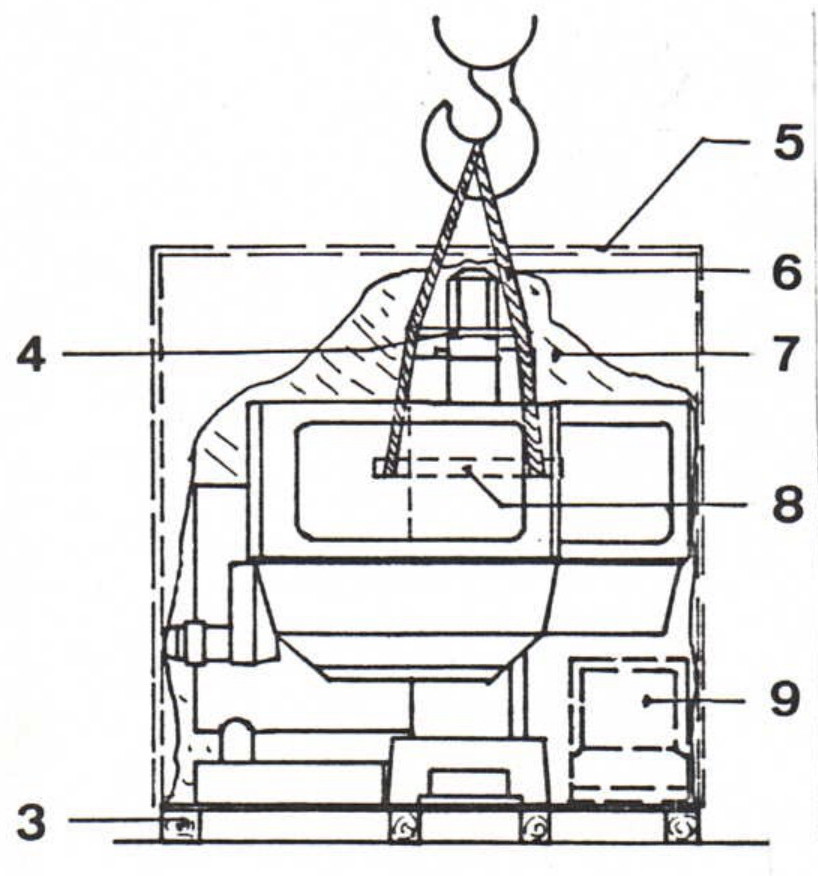
\includegraphics[width=\textwidth]{chapter1/machine_packaging_transport.jpg} % Replace with actual image file
        \caption{}
        \label{fig:packaging}
    \end{minipage}
    \hfill
    \begin{minipage}[b]{0.55\textwidth} % Align to the bottom with [b]
        \centering
        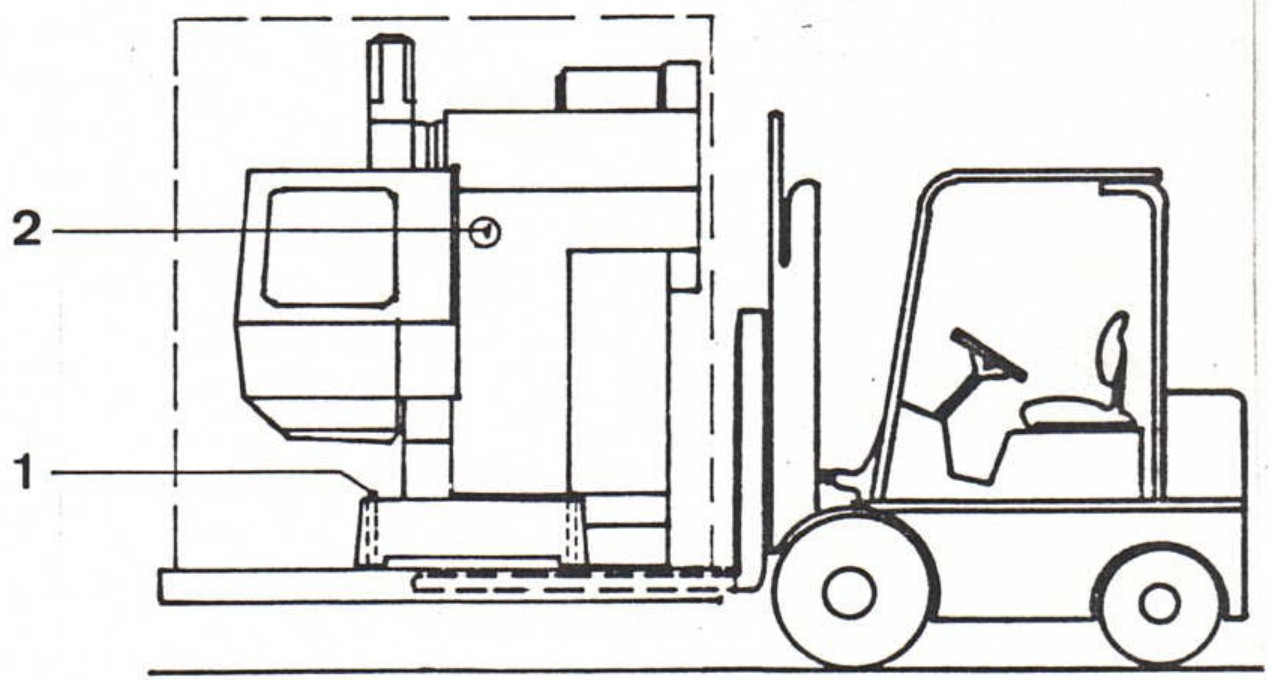
\includegraphics[width=\textwidth]{chapter1/machine_unloading_forklift.jpg} % Replace with actual image file
        \caption{}
        \label{fig:unloading}
    \end{minipage}
\end{figure}

\begin{itemize}
    \item Unload the packaged machine from the transport device using a forklift, hoist, or similar equipment.
    \item Remove the packaging (\textbf{5}) and cut and remove the protective foil (\textbf{7}) from the base of the box. Take off the sealing covers (\textbf{2}) on both sides.
    \item Check the machine and accessories for any transport damage.
\end{itemize}

\notebox{NOTE}{Damages or other defects, such as incompleteness, must be reported immediately in writing to the shipping company or railway, the insurance company, and the company MAHO.} 

\begin{itemize}
    \item Insert the transport rod (\textbf{8}) (maximum 50 mm diameter, 1000 mm length) into the opening in the stand.
    \item Attach the endless sling (\textbf{6}), with a minimum load capacity of 3000 kg and a total length of approximately 6 m, to the crane hook and the transport rod.
\end{itemize}

\notebox{CAUTION}{Place the detached control panel (\textbf{9}) on the work table and secure it against slipping!}

\sectionLikeSubsection{Transport of the Machine}

\begin{itemize}
    \item Perform a hanging test, i.e., align the machine by moving the transport rod (\textbf{8}) in the stand so that it hangs horizontally. Using a spacer (\textbf{4}) prevents the rope from rubbing against the machine.
    
    \item Lower the machine, unscrew the fastening nuts (\textbf{1}), and remove the pallet or box bottom (\textbf{3}) after lifting the machine again.
\end{itemize}

\textbf{When using a forklift:} Place the machine on wooden boards laid on the forks of the forklift (Fig. \ref{fig:unloading}) or hang it on the forks using a rope (Fig. \ref{fig:machine_placement_forklift}).
    
In unfavorable space conditions, use the "Transport Mule" (Fig. \ref{fig:machine_placement_mule}).

\begin{itemize}
    \item Transport the machine to the prepared location according to Page 1.03-1 and carefully place it on the damping plates provided.
\end{itemize}

\begin{figure}[h]
\centering
\begin{minipage}[t]{0.45\textwidth}
    \centering
    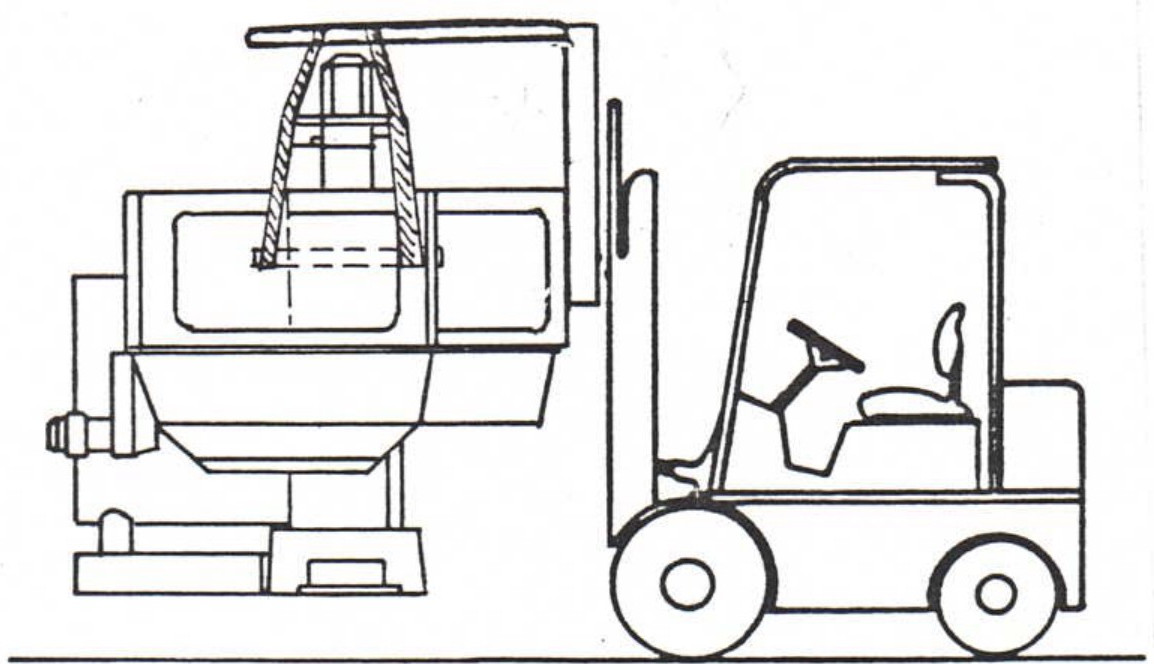
\includegraphics[width=\textwidth]{chapter1/machine_placement_forklift.jpg} % Replace with actual image file
    \caption{}
    \label{fig:machine_placement_forklift}
\end{minipage}
\hfill
\begin{minipage}[t]{0.45\textwidth}
    \centering
    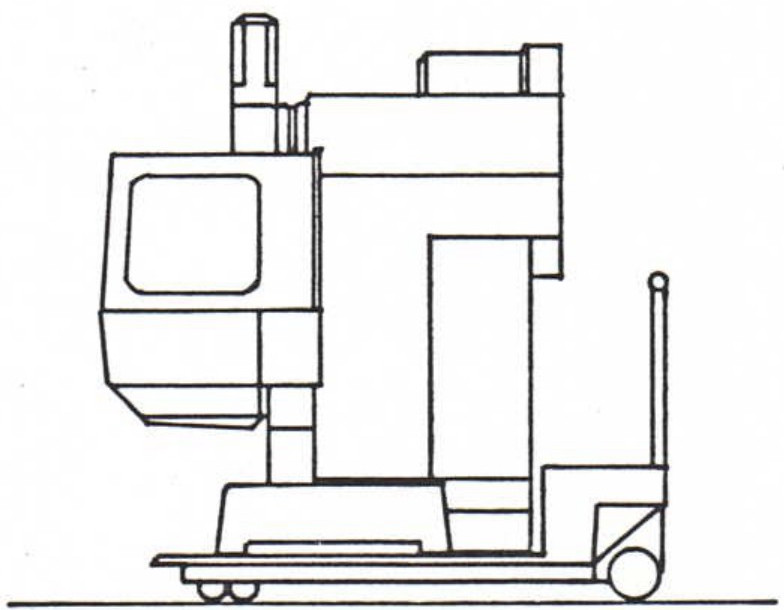
\includegraphics[width=\textwidth]{chapter1/machine_placement_mule.jpg} % Replace with actual image file
    \caption{}
    \label{fig:machine_placement_mule}
\end{minipage}
\end{figure}

\vspace{1em}

\infoBullet{Setup plan and workspace layout}{1.04-1}

\section{Installation of the Machine}

\subsection{Installation Site}
To ensure proper functionality of the machine, the following points regarding the installation site must be observed:
\begin{itemize}
    \item It must be free from vibrations.
    \item It must be free from local, one-sided heating or cooling of the machine, e.g., sunlight, radiators, drafts, etc.
    \item It must be free from interfering electrical installations (high-frequency).
    \item The total floor area requirement ($A_\text{WMP}$) is $3.2 \times 3.4 \, \text{m}$ ($10.88 \, \text{m}^2$).
    \item Within this total area, the machine covers an area of $3.5 \, \text{m}^2$, for which a minimum load-bearing capacity of $400 \, \text{daN/m}^2 \, (0.40 \, \text{t/m}^2)$ must be ensured.
    \item Ideally, the floor should be concrete or wood block.
\end{itemize}

\notebox{CAUTION}{
Mixed floors, i.e., machine standing on both concrete and wood block, are not permissible.
}

\begin{itemize}
    \item The unevenness of the floor must not exceed $3 \, \text{mm/m}^2$.
    \item A constant room temperature of max. $30^\circ \text{C}$ ($303 \, \text{K}$) must not be exceeded.
    \item The relative humidity must not exceed $80\%$.
\end{itemize}

\notebox{NOTE}{
Higher humidity or room temperatures up to $55^\circ \text{C}$ ($328 \, \text{K}$) are permissible when using MAHO cooling units in the command station and control cabinet.
}

\infoBullet{Setup plan and workspace layout}{1.04-1}\\
\infoBullet{Dimensions of the machine}{1.05-1}

\newpage
\sectionLikeSubsection{Setup of the Machine}

\begin{itemize}
    \item Lay out the supplied \enquote{Airlock damping plates} (1) according to the following sketch.
    \item Carefully place the machine on the damping plates.
    \item Leveling in the Z-direction (using shims) is necessary to ensure the oil level in the spindle head is maintained accurately!
    \item Position the coolant tank (2) accordingly, and screw the coolant pump (3) and return line (5) into the tank lid (4).
\end{itemize}

\vspace{1cm}

\begin{figure}[h!]
    \centering
    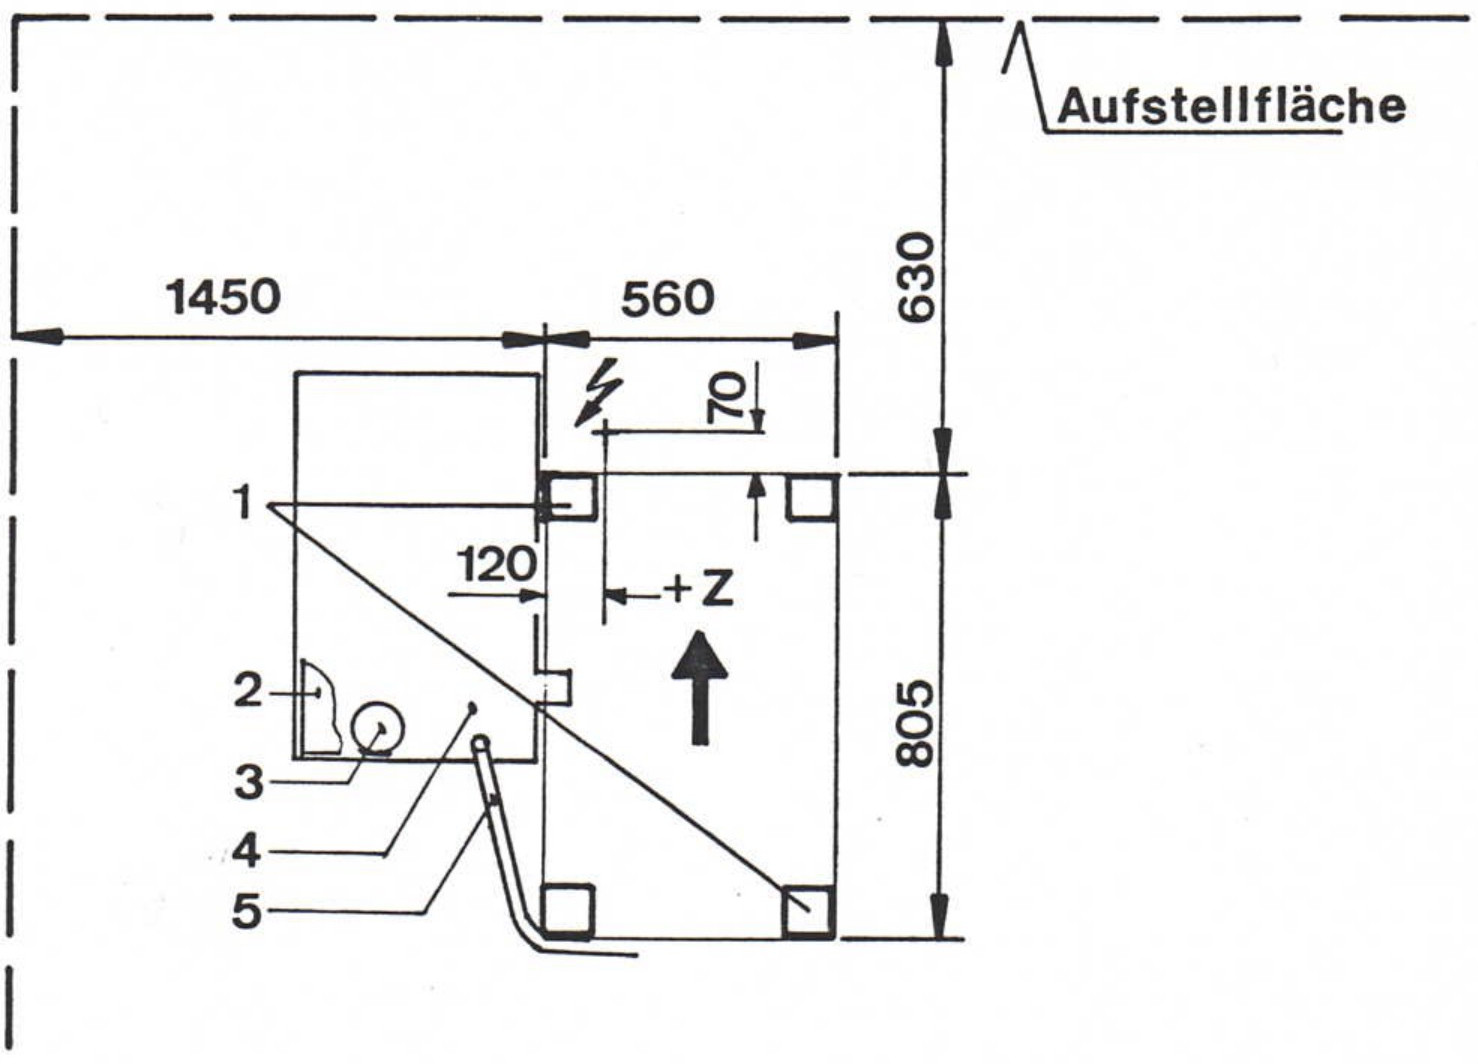
\includegraphics[width=\textwidth]{chapter1/machine_setup_sketch.jpg}
    \caption{Sketch for machine setup, including leveling and coolant system placement.}
    \label{fig:machine_setup_sketch}
\end{figure}

\sectionLikeSubsection{Mounting the Control Panel}

\begin{itemize}
    \item Remove the cover (7) and, if necessary, (9).
    \item Pull the pivot pin (8) out of the support (14).
    \item Place the extension arm (11) onto the support (14), slide the fork end \\(11.1) over the stop screw (12), and insert the cable bundle (13) into the bottom opening of the extension arm (11).
    \item Insert the pivot pin (8) into the extension arm (11) and the support (14). Tighten the mounting bracket of the cable hose (15) \\onto the extension arm.
    \item Insert the control panel (5) into the extension arm (11).
\end{itemize}

\begin{figure}[h!]
    \centering
    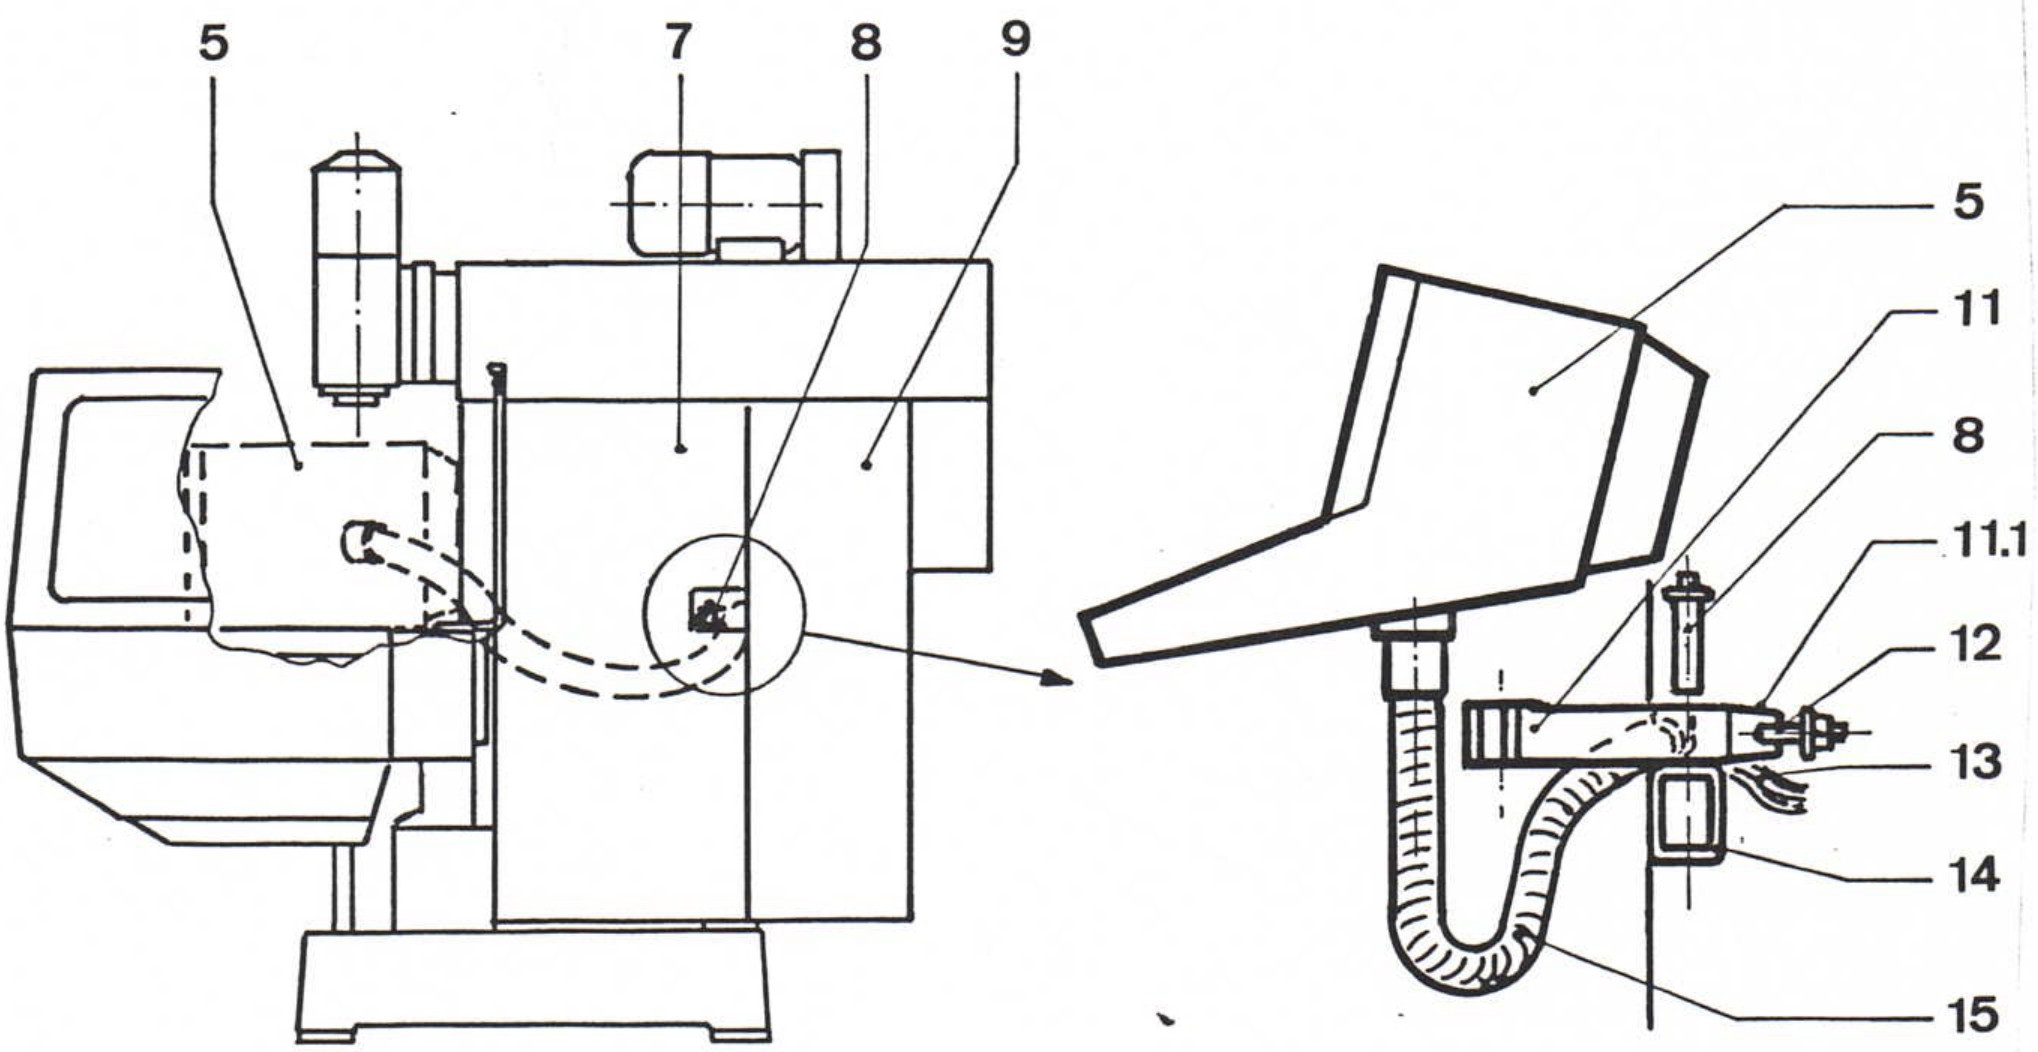
\includegraphics[width=\textwidth]{chapter1/control_panel_mounting_diagram.jpg}
    \caption{}
    \label{fig:control_panel_mounting}
\end{figure}

\section{Setup Plan and Workspace Layout}

\begin{description}[labelwidth=4cm, labelindent=0cm, leftmargin=0cm, rightmargin=2cm]
    \item[Total space requirement:] \dotfill 10.5 m\textsuperscript{2}
    \begin{itemize}
        \item Area for maintenance and disassembly \dotfill 5.06 m\textsuperscript{2}
        \item Machine footprint \dotfill 0.42 m\textsuperscript{2}
        \item Operator space \dotfill 3.8 m\textsuperscript{2}
        \item Setup area \dotfill 1.6 m\textsuperscript{2}
        \item Coverage area (F) \dotfill 3.25 m\textsuperscript{2}
    \end{itemize}
    \item[Height of the machine:] \dotfill 1.83 m
    \item[Weight of the machine (total):] \dotfill approx. 1,250 kg
    \item[Floor load on area (F):] \dotfill approx. 400 kg/m\textsuperscript{2}
\end{description}

\begin{figure}[H]
    \centering
    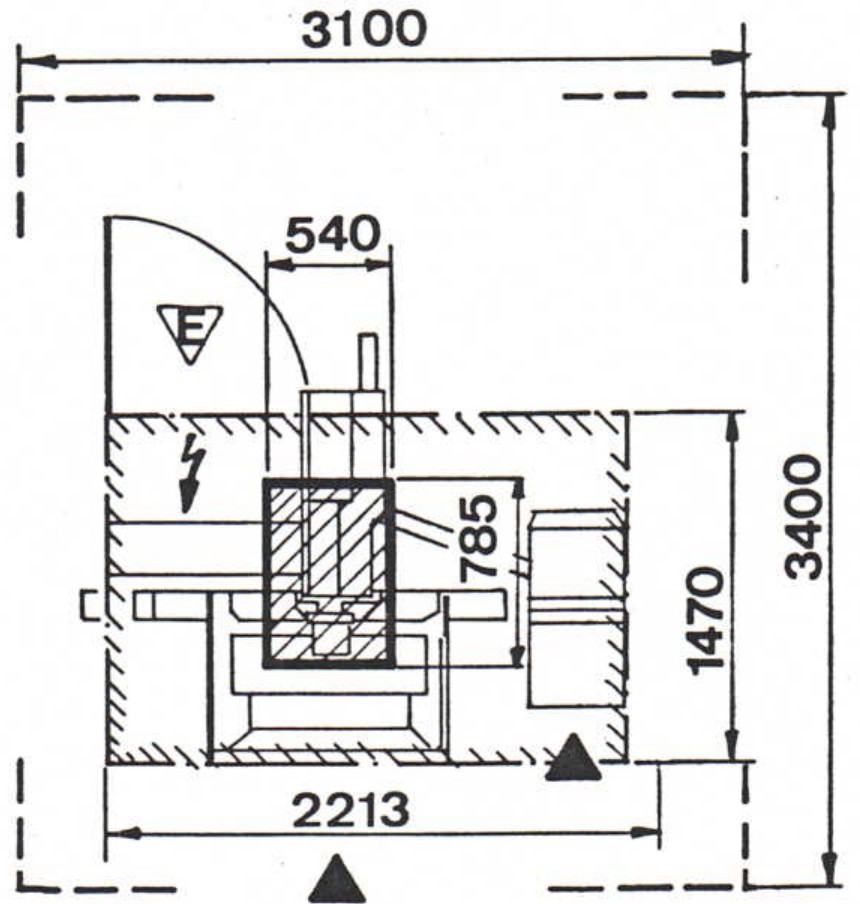
\includegraphics[width=0.45\textwidth]{chapter1/setup_plan_workspace_layout_diagram.jpg}
    \caption{}
    \label{fig:setup_plan_workspace_layout}
\end{figure}

\begin{description}[labelwidth=0cm, labelindent=0cm, leftmargin=0cm]
    \item \adjustbox{valign=c}{
\includegraphics[height=1cm]{chapter1/icon_electrician_access.jpg}} \hspace{0.5cm} Electrician access
    \item \adjustbox{valign=c}{
\includegraphics[height=1cm]{chapter1/icon_coverage_area.jpg}} \hspace{0.5cm} Coverage area (F)
    \item \adjustbox{valign=c}{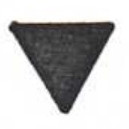
\includegraphics[height=1cm]{chapter1/icon_operator_position.jpg}} \hspace{0.5cm} Operator position
\end{description}

\vspace{-\topsep} % Suppress extra vertical space above the block
\begin{minipage}{\textwidth}
    \begin{minipage}[t]{1.5cm} % Adjust the width for the icon
        \raggedright
        \raisebox{-0.5\height}{% Adjust vertical alignment of the icon
            
\includegraphics[height=1cm]{chapter1/icon_electrical_connection.jpg}
        }
    \end{minipage}%
    \begin{minipage}[t]{\dimexpr\textwidth-1.5cm\relax} % Remaining space for text
        \begin{description}[labelwidth=6cm, labelindent=0cm, leftmargin=7cm, itemsep=0pt]
            \item[Power connection:] \dotfill 11 kVA
            \item[Free cable length across the floor:] \dotfill 0.5 m
            \item[Maximum fuse rating:] 
            \begin{itemize}[itemsep=0pt, topsep=0pt]
                \item 200-220 V \dotfill 35 A
                \item 380-500 V \dotfill 25 A
            \end{itemize}
        \end{description}
    \end{minipage}
\end{minipage}

\section{Dimensional Drawing of the Machine}

\begin{figure}[H]
    \centering
    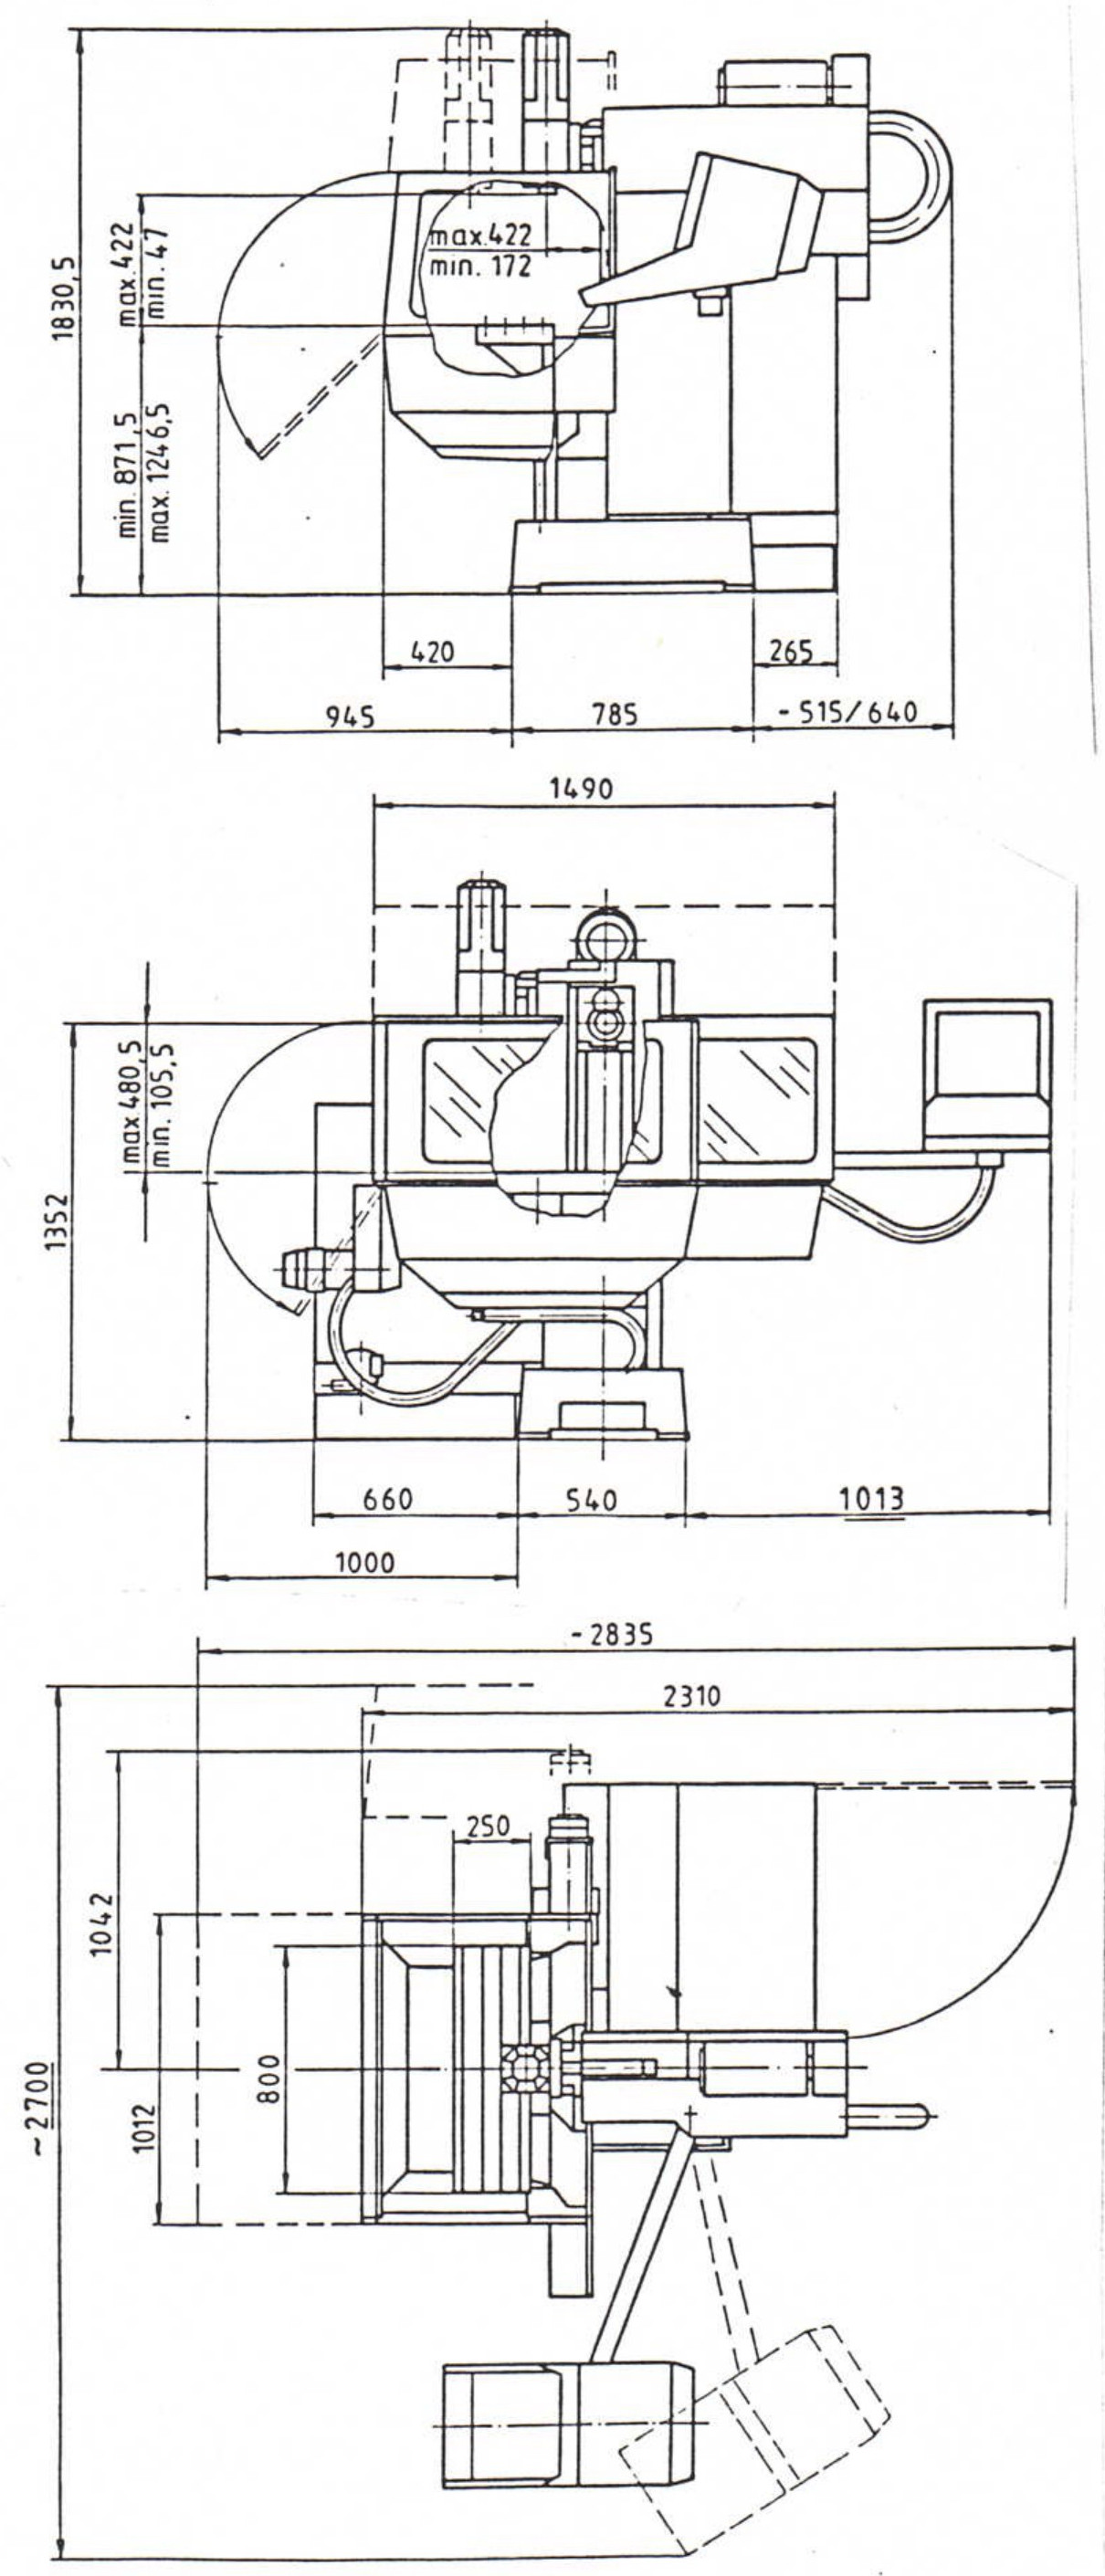
\includegraphics[width=.55\textwidth]{chapter1/machine_dimensions.jpg}
    \caption{}
    \label{fig:setup_plan_workspace_layout}
\end{figure}


\section{Removal of the Rust Protection Agent}

\setcounter{section}{8}

\notebox{WARNING}{Before removing the rust protection agent from the machine, no adjustments to the slides must be made.}

\begin{figure}[h]
    \centering
    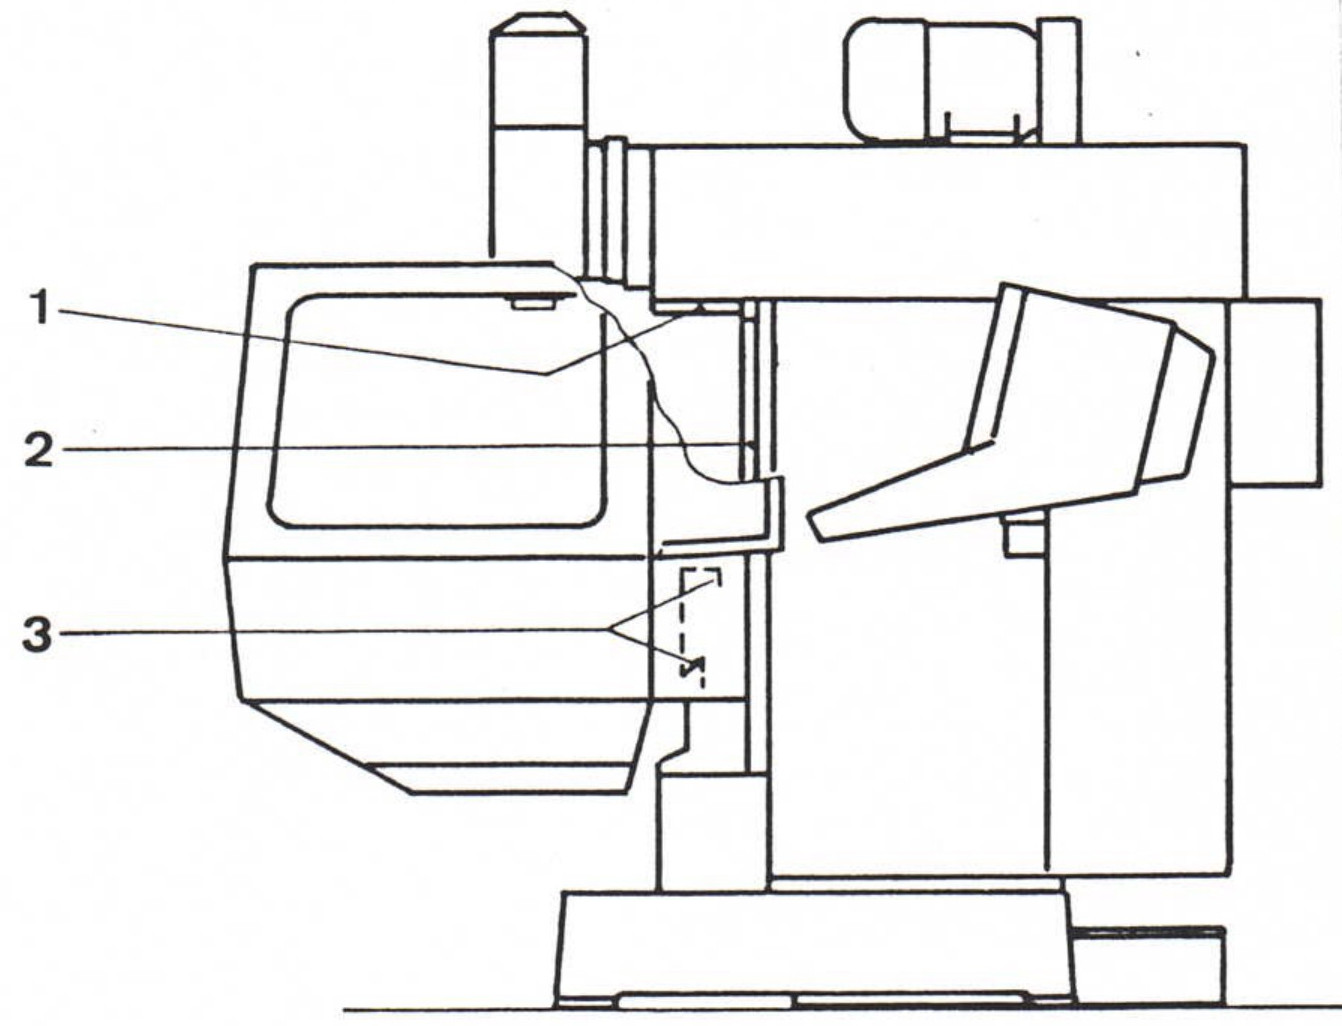
\includegraphics[width=0.7\textwidth]{chapter1/diagram_removal_of_rust_protection_agent.jpg}
    \caption{}
\end{figure}

\begin{itemize}
    \item Carefully remove the rust protection agent from the bare external surfaces and the receptacle cones of the work spindles using a soft cloth soaked with petroleum, gasoline, tetra, or another solvent for hydrocarbons.
    \item \textbf{Do not under any circumstances use scrapers or other sharp tools for this task.}
    \item Clean the sliding surfaces of the dovetail guides of the headstock (1) and the cross slide (2) with a soft cloth to remove the rust protection grease and apply oil with a brush.\footnotemark[2]
    \item Clean accessible sliding surfaces of the combined dovetail flat guides (3) of the vertical clamping table with a soft cloth to remove the rust\\ protection grease and apply oil.
\end{itemize}

\footnotetext[2]{The oil used in the central lubrication system must be applied (see page 7.06-1 \enquote{Lubricant Recommendations}).}

\notebox{WARNING}{Mixing of oils must be strictly avoided.}

\section{Filling the Drive Gear Oil Reservoir in the Spindle Head}

To prepare the machine for operation, the oil in the work spindle drive must be drained during transport and refilled before commissioning.

\vspace{.5cm}

\notebox{CAUTION}{Verify that the machine is level in the Z-axis using a spirit level, and adjust if necessary.\footnotemark[3]}

\footnotetext[3]{See Sheet 1.03-1.}

\begin{itemize}[itemsep=0.5em]
    \item Unscrew the front fill screw (1).
    \item Using the supplied container labeled "CLP 46/HLP 46" (Aral Sumorol CM 46), pour 0.2 liters into a measuring container and fill it into the fill opening (2) on the spindle head.
    \item Wait approximately 10 minutes, then read the oil level in the sight glass. If necessary, refill the remaining quantity in steps of 0.1 liters using the measuring container until the oil level reaches the corresponding mark (3).
    \item Reattach the fill screw (1).
\end{itemize}

\begin{figure}[h!]
    \centering
    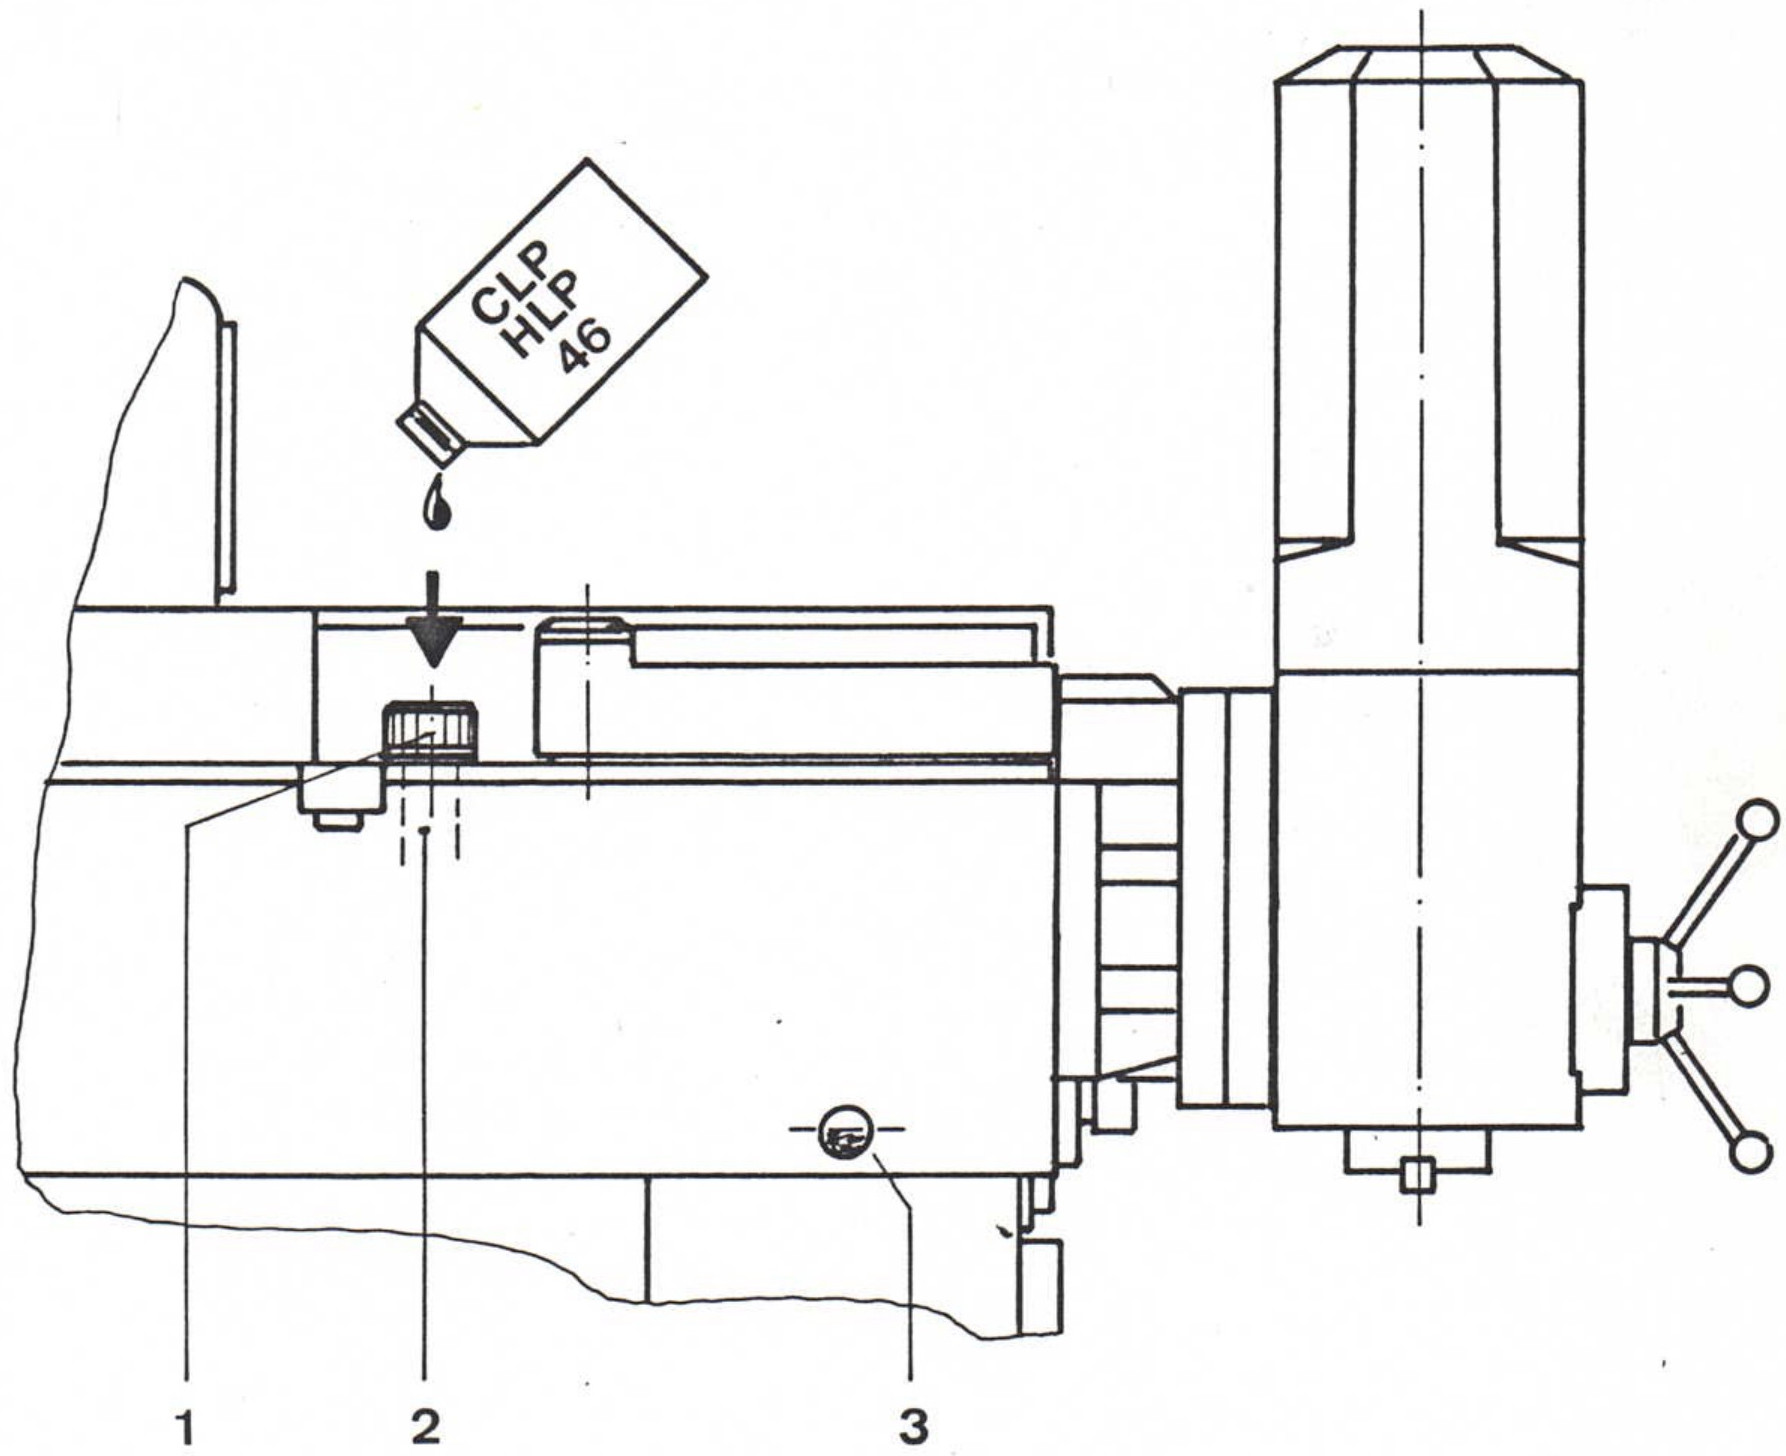
\includegraphics[width=0.8\textwidth]{chapter1/spindle_oil_fill_diagram.jpg} % Replace with your image filename
    \caption{}
\end{figure}


\section{Connecting to the Electrical Network}

Connection regulations from the responsible power supply company must be observed.

\begin{figure}[htp] % Top alignment for the figure
    \centering
    \begin{minipage}[t]{.4\linewidth} % Adjust the width for the image
        \centering
        \raisebox{-\height}{% Top-align the image
            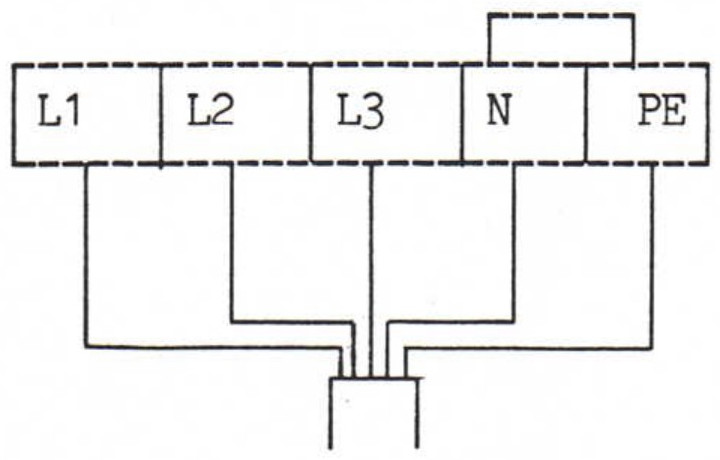
\includegraphics[width=\linewidth]{chapter1/electrical_connection_diagram.jpg}
        }
        \caption{Electrical connection diagram.} % Caption below the image
        \label{fig:electrical_connection} % Optional: add label for referencing
    \end{minipage}%
    \hfill % Add space between image and text
    \begin{minipage}[t]{\dimexpr\textwidth-8cm\relax} % Remaining width for the text
        \vspace{0pt} % Ensures top alignment of this minipage
        Total connection power: \dotfill 11 kVA \\\\
        Fuse, max.: \\
        200-220 V \dotfill 35 A \\
        380-500 V \dotfill 25 A
    \end{minipage}
\end{figure}

\begin{itemize}
    \item Switch off the main switch \textbf{-Q1-} on the control cabinet.
    \item Open the control cabinet door. Feed the connection cable through the \\provided opening and connect it to the input terminals L1, L2, L3, N, PE.
    \item For 4-pole connections, terminals N and PE must be bridged.
    \item Check the phase sequence using a phase sequence indicator on terminals L1, L2, L3. If necessary, swap two phases at the input terminals.
    \item Check all terminal screws on the terminal strips, contactors, relays, and fuses in the control cabinet for tightness.
    \item Only after establishing the correct phase sequence, switch on the main \\switch \textbf{-Q1-} on the control cabinet and perform a function test following the instructions on Page 3.01-1.
\end{itemize}

\notebox{NOTE}{The electrical documentation is located in a pocket on the inside of the control cabinet door and must remain in the machine!}

\notebox{CAUTION}{When connecting peripheral devices (reader-puncher, corner milling head, grinding head), check the voltage of the socket.}

Fuses must only be replaced with equivalent types.

Adjustment values on potentiometers, adjustment switches, machine parameters, etc., must only be changed by service personnel.

\section*{Commissioning Checklist}

Before starting the working spindles and axis movements, the following points must be completed:

\begin{enumerate}
    \item Proper setup, see page 1.03-1.
    \item Rust protection removed, see page 1.08-1.
    \item Oil bath filled, see page 1.09-1.
    \item Electrical connection, see page 1.10-1.
\end{enumerate}

\end{document}